\documentclass[conference,onecolumn]{IEEEtran}
\usepackage{enumitem}
%\usepackage{cite}
\usepackage{graphicx}
\usepackage{float}
\usepackage{amsmath, nccmath, bm}
\usepackage{amssymb}
\graphicspath{{./images}}
\usepackage[backend=biber,style=numeric]{biblatex}
\addbibresource{sources.bib}


\begin{document}
\section{Time Interleaver}
\subsection{Time Interleaver Overview}
XM requires time diversity in its services to ensure a minimum dropout for paying customers.  To accomplish this, XM uses a convolutional time interleaver to spread the transmitted bits over a wide time (specifically 4.69 seconds).  Time diversity allows the receiver to recover the transmitted signal with large signal blockage time. 

\subsection{Time Interleaver XM}
In the XM radio MFP structure, the data is partitioned into 258 prime rate channels (PRCs) that are grouped in blocks of 5440 transmitted bits  as seen in Figure {CITE MFP/FSP}.  These 5440 bit PRCs are the results of the FEC encoding which uses a RS(255,223) block code (Reed Solomon) followed by a convolutional encoding at rate 3/8.  A RS(255,223) encoder produces 2040 transmitted bits and the rate 3/8 convolution encoding increases the transmitted bits to 5440.  Each satellite transmits 1/2 the bits or 2720 bits.  Details of the FEC encoding will follow in FEC section.\\
Each PRC of 5440 bits per satellite is equal to 2 RS codewords.  Figure \ref{fig::time_interleaver} obtained from {CITE XM PATENT}, shows XM using a separate convolutional time interleaver on each PRC \\

\begin{figure}[H]
	\centerline{\fbox{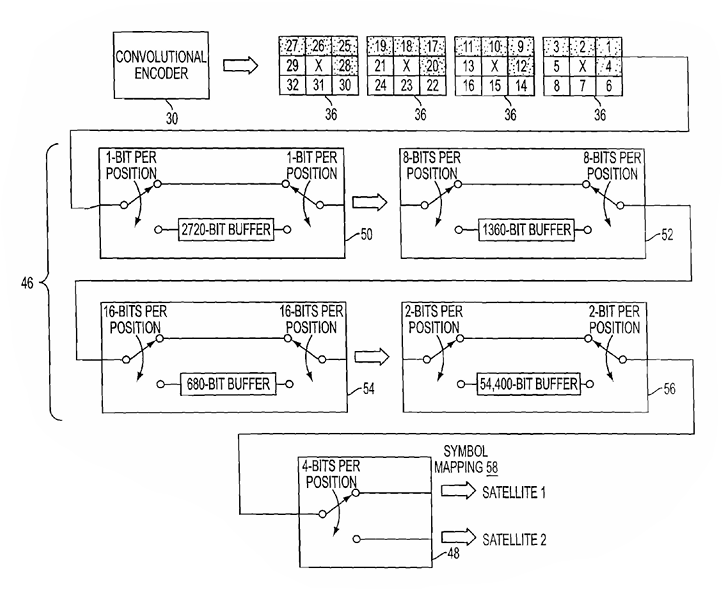
\includegraphics[width=0.8\textwidth]{XM_TIME_INTERLEAVER_DETAILS_no_label.png}}}
	\caption{XM Time Interleaver}
	\label{fig::time_interleaver}
\end{figure}
Figure \ref{fig::time_interleaver} shows the time interleaver from the transmission point of view.  The receiver follows in reverse. As can be seen each satellite can be processed independently or combined in a receiver through this time interleaver mechanism.  For the test, a single satellite (sat2) was used as the source and inserted zeros for the other satellite (sat1). Highlighted in block 36 is the punctured bits marked by an X and satellite 1 bits 1-4 and satellite 2 bits 5-8.  As can be seen in Figure \ref{fig::time_interleaver}, when one uses 5440 bits per MFP (0.432 ms) and calculates the maximum delay through the 4 buffers, the result is an interleaver delay of 4.698 seconds described in the XM chipset STA400a section 1.4 TDM DECODING {CITE}.

\section{Convolutional Decoder}
\subsection{Convolutional Decoder Overview}
A convolutional encoder/decoder uses a concept similar to FIR/IIR filters where the information bits are spread over time using GF(2).  These codes have been around since the 1950's.  These codes use registers to keep track of the state of the system.  They can be both recursive and non-recursive feedback polynomials to spread the information bits across time.  Non-recursive convolutional codes are commonly decoded with the Viterbi algorithm and recursive polynomials are commonly used in Turbo codes.

\subsection{Convolutional Decoder XM}
XM uses a non-recursive convolutional encoder/decoder as part of the concatenated coding.  Concatenated codes typically use an inner convolutional code with an outer block code.  For the XM system, they employ a complementary convolutional encoder.  This is a way to split the transmitted information across the two satellites as well as the terrestrial signal.  Figure \ref{fig::Viterbi} shows details of the convolution encoder described in XM patent {cite}.  This encoder takes in 3 information bits and creates 9 transmitted bits.  The bits labeled ``A'', ``B'', ``C'' and ``D'' are sent to satellite 1 and bits ``F'', ``G'', ``H'' and ``J'' are sent to satellite 2.  The terrestrial signal uses the same bits as satellite 2 with the addition of bit ``E''.\\

Combining Figure \ref{fig::time_interleaver} and Figure \ref{fig::Viterbi} describe the convolutional encoding, bit puncturing and time interleaving of the XM system.
\begin{figure}[H]
	\centerline{\fbox{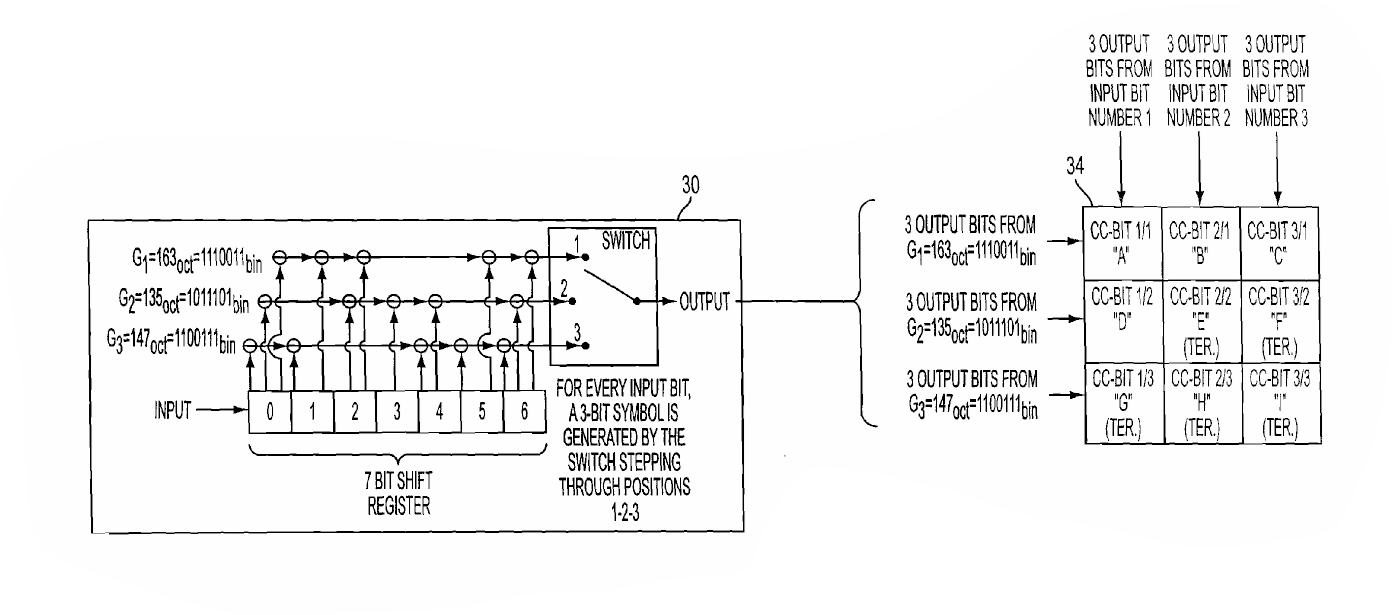
\includegraphics[width=0.8\textwidth]{Viterbi_encoder.png}}}
	\caption{XM Convolutional Encoder}
	\label{fig::Viterbi}
\end{figure}
\subsection{Procedure}  Taking the MFP aligned blocks, the first PRC (5440 bits) of satellite 2 was extracted following the description of the time interleaver.  The STA400a chipset and related patents mention a Time Slot Control Channel (TSCC) as the first set of PRCs which should contain a frame counter.  This was chosen as the best PRC to use as the channel structure is not expected to change constantly through a shorter time frame.  Since only one satellite was used, multiple frames were processed through the time interleaver to accumulate enough bits for testing with a Matlab Viterbi decoder.  With a single satellite, one can use either the top portion of the Viterbi decoder or the bottom portion depending on the chosen satellite.  With both satellites, the Viterbi is run at a rate 1/3 code rate.  When using a single satellite, the Viterbi decoder operates at an effective code rate of 1/2 with correct puncturing. This corresponds to a 3/4 encoder rate—meaning that for every 4 received bits, 3 are usable as information bits.  The decoder however, consistantly needs more than 3 transmission bits in order to determine the state of the trellis.

\begin{figure}[H]
	\centerline{\fbox{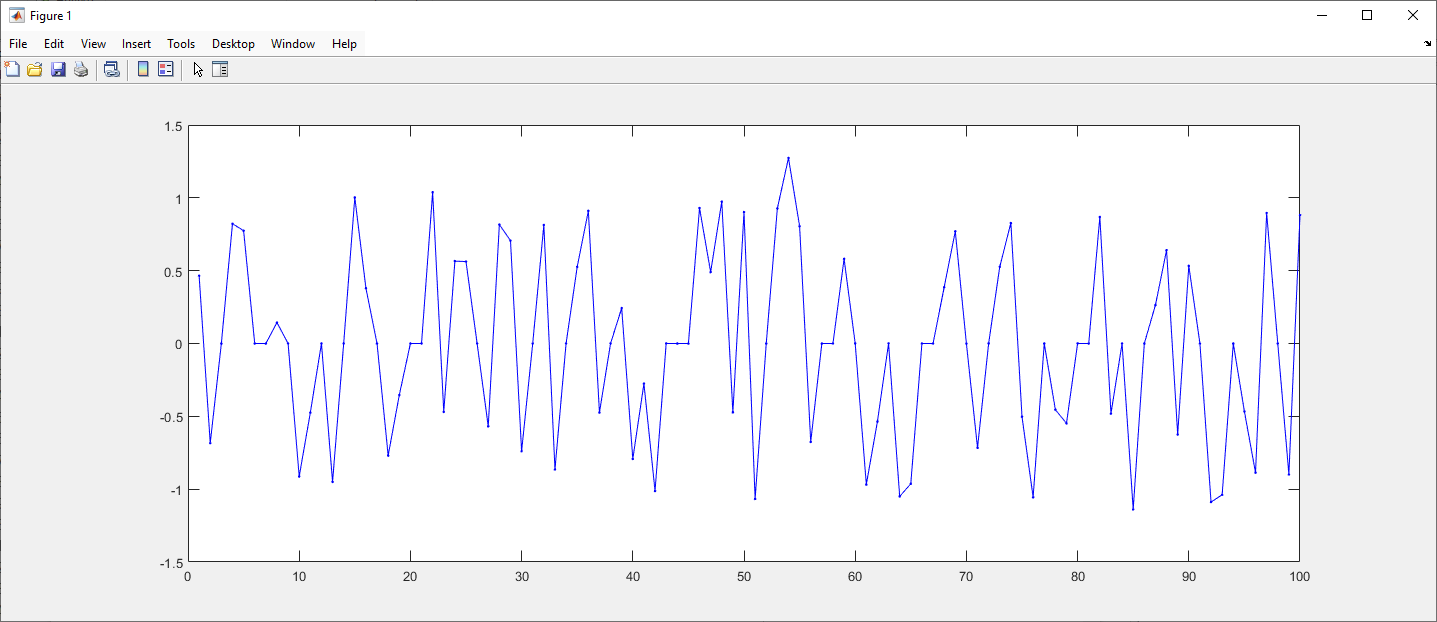
\includegraphics[width=0.8\textwidth]{Viterbi_insufficient_bits.png}}}
	\caption{XM Insufficient Data into Decoder}
	\label{fig::Viterbi_1}
\end{figure}
\begin{figure}[H]
	\centerline{\fbox{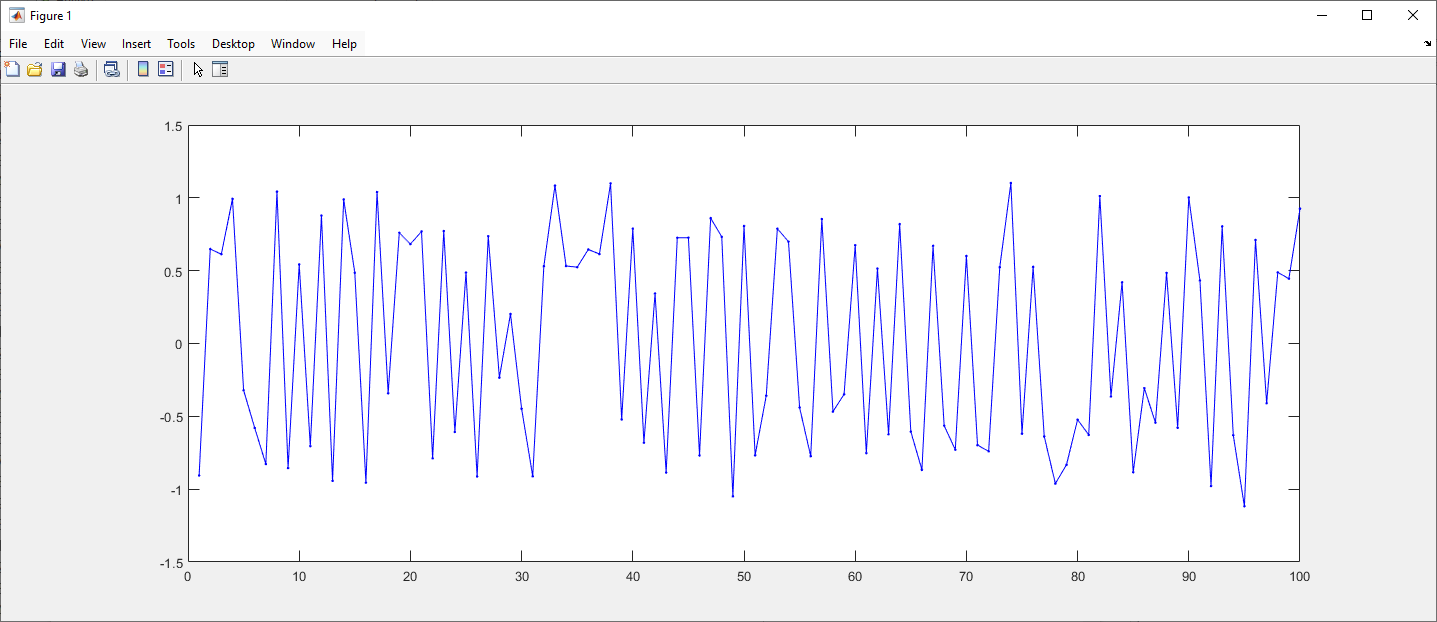
\includegraphics[width=0.8\textwidth]{Viterbi_sufficient_bits.png}}}
	\caption{XM Sufficient Data into Decoder}
	\label{fig::Viterbi_2}
\end{figure}

In Figure \ref{fig::Viterbi_1}, there is an insufficient number of input bits to a Viterbi decoder as the time interleaver is not completely full.  Since we are only using 1 satellite, the FEC is not capable of decoding this PRC block.  In Figure \ref{fig::Viterbi_2}, which is later in time, there is sufficient transmitted bits to use in the Viterbi decoder.\\

Next we looked at the Viterbi output for satellite 2.  This was done using the Matlab SPY plot.  As can be seen in Figure \ref{fig::Viterbi_spy}, the output shows no structure in the vertical domain and lacks the expected frame counter.  
\begin{figure}[H]
	\centerline{\fbox{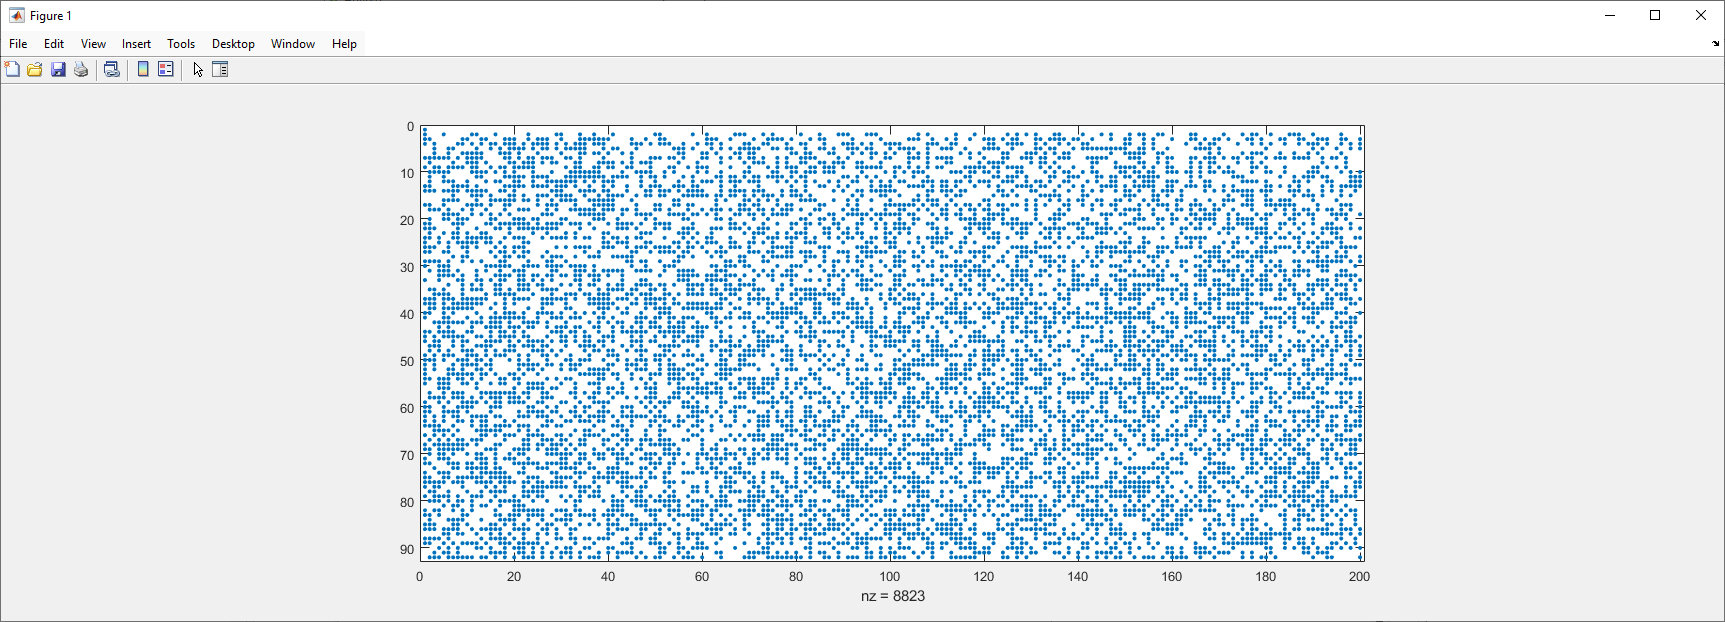
\includegraphics[width=0.8\textwidth]{Viterbi_SPY.png}}}
	\caption{XM Viterbi SPY Output}
	\label{fig::Viterbi_spy}
\end{figure}
At this point we re-examined the documentation and discovered that the STA400a chipset showed a potential scrambler.  This was not included in any patent descriptions, not any mention in the STA400a document of the scrambler implementation.  Resolving this unknown scrambler was outside the scope of the project.  A scrambler is sometimes used in digital communication systems to disperse energy so the timing and carrier recovery algorithms have transitions in the received symbols.  These are typically done with Linear Feedback Shift Registers (LFSR) and create a pseudo random sequence that is added to the original codeword in GF(2) space prior to transmission.  By applying the same pseudo random sequence at the receiver, the scrambling is removed.  This would be done between the timing/carrier recovery algorithm and FEC algorithm.\\

The absence of a descrambler would explain why no recognizable frame structure was observed in the Viterbi output, despite correct decoding procedures.  There was also mention of a RS block interleaver that was also undocumented except overview descriptions in the STA400a chipset.  Resolving the descrambler is required prior to resolving the block interleaver algorithm. 

\begin{figure}[H]
	\centerline{\fbox{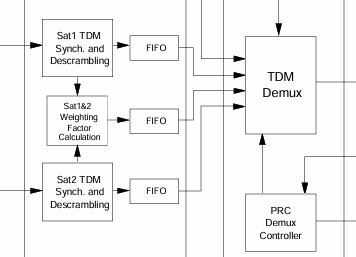
\includegraphics[width=0.8\textwidth]{XM_scrambler.png}}}
	\caption{XM potential scrambler}
	\label{fig::scrambler}
\end{figure}


\end{document}
